\documentclass[aspectratio=169, 11pt]{beamer}
\usepackage{fontspec}
\setmainfont{TeX Gyre Termes}
\setsansfont{TeX Gyre Heros}
\setmonofont{Latin Modern Mono}
\usepackage[spanish,es-nodecimaldot]{babel}
\usepackage{amsmath, amssymb, amsfonts, booktabs, graphicx}
\usepackage{tikz}
\usetikzlibrary{shapes.geometric, arrows.meta, positioning, calc, fit, shadows}
\usetheme{Madrid}
\usecolortheme{beaver}
\definecolor{unalRojo}{RGB}{148, 36, 36}
\definecolor{verdeOK}{RGB}{34, 139, 34}
\definecolor{naranjaAlerta}{RGB}{230, 126, 34}
\definecolor{rojoAlerta}{RGB}{192, 57, 43}
\definecolor{azulReactor}{RGB}{41, 128, 185}
\definecolor{verdeEntrada}{RGB}{39, 174, 96}
\setbeamercolor{structure}{fg=unalRojo}
\setbeamercolor{block title}{bg=unalRojo!15, fg=unalRojo}
\setbeamercolor{block body}{bg=unalRojo!5}
\setbeamercolor{alerted text}{fg=rojoAlerta}
\newcommand{\BSF}{\textit{Hermetia illucens}}
\newcommand{\MAPE}{\text{MAPE}}
\newcommand{\NDIR}{\text{NDIR}}
\newcommand{\MRV}{\text{MRV}}
\setbeamertemplate{navigation symbols}{}
\setbeamertemplate{footline}[frame number]

\begin{document}

% ---------------------------------------------------------------------------
% Slide 1: Pregunta 2
% ---------------------------------------------------------------------------
\begin{frame}{Arquitectura h\'{i}brida y MRV}
    \begin{center}
        \begin{tikzpicture}
            \node[rectangle, rounded corners=5pt, draw=unalRojo, fill=unalRojo!5, 
                  text width=14cm, align=justify, inner sep=12pt, font=\small] at (0,0) {
                \textbf{?`De qu\'{e} manera la arquitectura h\'{i}brida (sens\'{o}rica IoT, modelo f\'{i}sico e IA) permite pasar de esquemas basados en factores de emisi\'{o}n est\'{a}ticos a un enfoque din\'{a}mico de cuantificaci\'{o}n, trazabilidad y detecci\'{o}n de eventos cr\'{i}ticos en la bioconversi\'{o}n con \BSF?}
            };
        \end{tikzpicture}
    \end{center}
\end{frame}

% ---------------------------------------------------------------------------
% Slide 2: Pregunta 4
% ---------------------------------------------------------------------------
\begin{frame}{Calibraci\'{o}n NDIR y m\'{e}tricas}
    \begin{center}
        \begin{tikzpicture}
            \node[rectangle, rounded corners=5pt, draw=unalRojo, fill=unalRojo!5, 
                  text width=14cm, align=justify, inner sep=12pt, font=\small] at (0,0) {
                \textbf{Explique c\'{o}mo la calibraci\'{o}n de sensores \NDIR{} de bajo costo influye en la calidad de las estimaciones de CO$_2$ y CH$_4$. ?`Qu\'{e} m\'{e}tricas deben utilizarse para evaluar el desempe\~{n}o frente a instrumentos de referencia?}
            };
        \end{tikzpicture}
    \end{center}
\end{frame}

% ---------------------------------------------------------------------------
% Slide 3: De est\'{a}tico a din\'{a}mico
% ---------------------------------------------------------------------------
\begin{frame}{De factores est\'{a}ticos a cuantificaci\'{o}n din\'{a}mica}
    \begin{columns}[T]
        \begin{column}{0.48\textwidth}
            \begin{alertblock}{El problema de lo est\'{a}tico}
                \begin{itemize}
                    \item Supone que el proceso siempre se comporta igual.
                    \item Promedios fijos del IPCC o compostaje no reflejan la realidad horaria.
                    \item Subestima picos de CH$_4$ y desv\'{i}a balances de carbono.
                \end{itemize}
            \end{alertblock}
        \end{column}
        \begin{column}{0.48\textwidth}
            \begin{block}{El enfoque din\'{a}mico}
                \begin{itemize}
                    \item Serie temporal continua (minuto a minuto).
                    \item Factor de emisi\'{o}n ajustado por condiciones operativas del momento.
                    \item Curva espec\'{i}fica por cada lote de residuos tratado.
                \end{itemize}
            \end{block}
        \end{column}
    \end{columns}
\end{frame}

% ---------------------------------------------------------------------------
% Slide 4: Arquitectura h\'{i}brida (con imagen)
% ---------------------------------------------------------------------------
\begin{frame}{Arquitectura h\'{i}brida: IoT $\rightarrow$ Modelo f\'{i}sico $\rightarrow$ IA}
    \begin{center}
        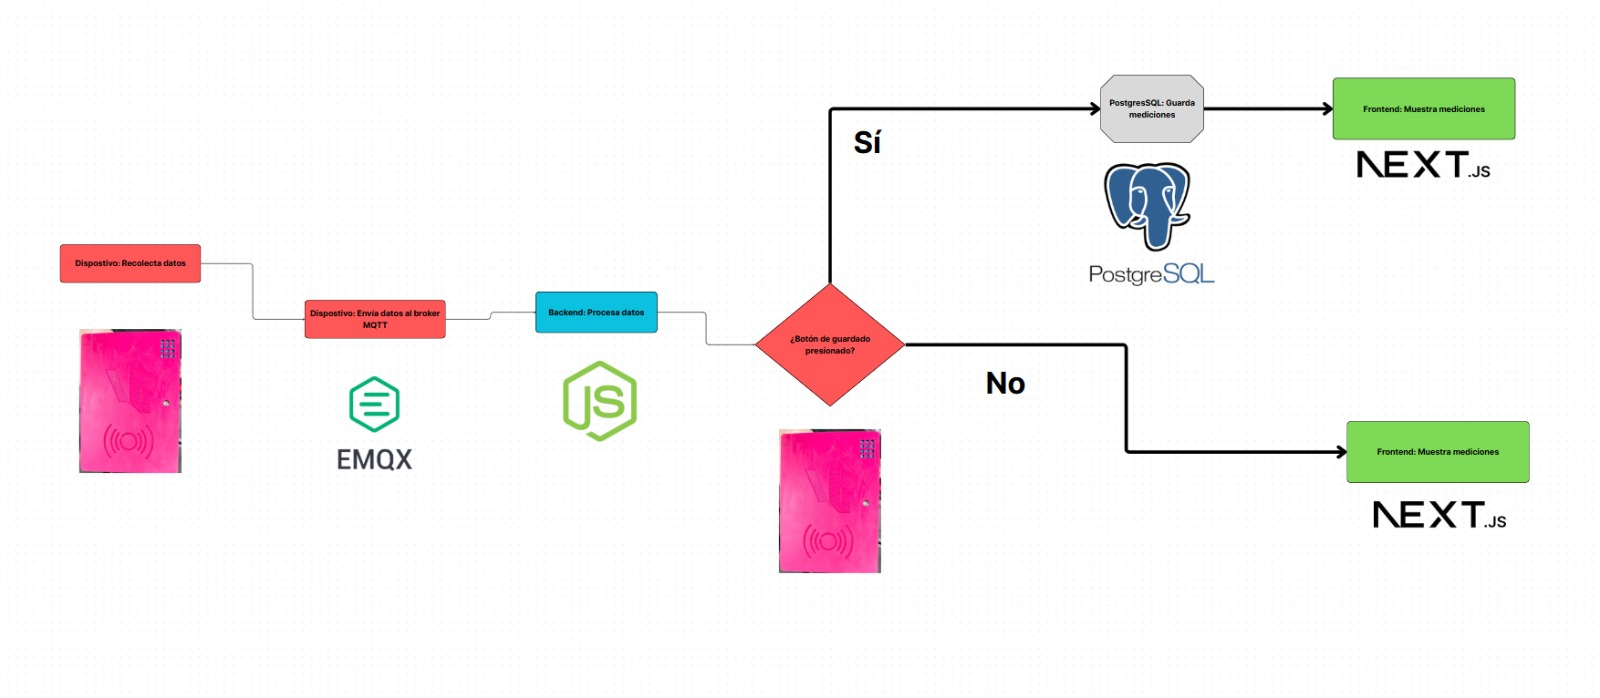
\includegraphics[width=0.82\textwidth]{esquema.jpeg}
    \end{center}
\end{frame}

% ---------------------------------------------------------------------------
% Slide 5: Sensores y edge computing
% ---------------------------------------------------------------------------
\begin{frame}{Instrumentaci\'{o}n: sensores NDIR Windsent y edge computing}
    \begin{columns}[T]
        \begin{column}{0.55\textwidth}
            \begin{block}{Sensores NDIR de foco}
                \begin{itemize}
                    \item \textbf{Winsen MH-410D}: CO$_2$ (NDIR, bajo costo).
                    \item \textbf{Winsen MH-441D}: CH$_4$ (NDIR, bajo costo).
                    \item Calibraci\'{o}n peri\'{o}dica con gases patr\'{o}n certificados.
                    \item Correcci\'{o}n multivariable: T, HR, presi\'{o}n.
                \end{itemize}
            \end{block}
        \end{column}
        \begin{column}{0.42\textwidth}
            \begin{block}{Edge computing}
                \begin{itemize}
                    \item Procesamiento local en el nodo sensor.
                    \item Reducci\'{o}n de latencia y dependencia de nube.
                    \item Continuidad ante p\'{e}rdida de conectividad.
                \end{itemize}
            \end{block}
        \end{column}
    \end{columns}

    \vfill
    \begin{center}
        \footnotesize
        Variables de contexto (no foco): NPK, pH, humedad/temperatura de biomasa y ambiente, conductividad el\'{e}ctrica.
    \end{center}
\end{frame}

% ---------------------------------------------------------------------------
% Slide 6: Trazabilidad MRV
% ---------------------------------------------------------------------------
\begin{frame}{Trazabilidad MRV: de la medici\'{o}n al cr\'{e}dito de carbono}
    \begin{center}
        \begin{tikzpicture}[scale=0.85, transform shape,
            capa/.style={rectangle, rounded corners=5pt, draw=azulReactor, fill=azulReactor!10, minimum width=2.6cm, minimum height=1.2cm, align=center, font=\small},
            flecha/.style={-{Stealth}, line width=2pt, azulReactor}]

            \node[capa] (sens) at (-6,0) {Sensor\\marca de tiempo + ID};
            \node[capa] (mod) at (-2,0) {Modelo f\'{i}sico\\validaci\'{o}n biol\'{o}gica};
            \node[capa] (ia) at (2,0) {IA (PINN)\\ajuste din\'{a}mico};
            \node[capa] (rep) at (6,0) {Reporte\\auditable};

            \draw[flecha] (sens.east) -- (mod.west);
            \draw[flecha] (mod.east) -- (ia.west);
            \draw[flecha] (ia.east) -- (rep.west);
        \end{tikzpicture}
    \end{center}

    \vfill
    \begin{itemize}
        \item Cada dato lleva: timestamp, ID del sensor, nota de calibraci\'{o}n, par\'{a}metros operativos.
        \item El auditor reconstruye paso a paso c\'{o}mo se obtuvo cada cifra.
        \item Requisito exigido por VCS, Gold Standard y Art\'{i}culo 6 del Acuerdo de Par\'{i}s.
    \end{itemize}
\end{frame}

% ---------------------------------------------------------------------------
% Slide 7: Detecci\'{o}n de eventos
% ---------------------------------------------------------------------------
\begin{frame}{Detecci\'{o}n de eventos cr\'{i}ticos}
    \begin{center}
        \begin{tikzpicture}[scale=0.85, transform shape,
            paso/.style={rectangle, rounded corners=5pt, draw=rojoAlerta, fill=rojoAlerta!8, minimum width=3.4cm, minimum height=1.2cm, align=center, font=\small},
            flecha/.style={-{Stealth}, line width=2pt, rojoAlerta}]

            \node[paso] (sen) at (-4.5,0) {Sensor detecta\\CH$_4$ inesperado};
            \node[paso] (mod) at (0,0) {Modelo aerobio\\predice CO$_2$ s\'{o}lo};
            \node[paso] (res) at (4.5,0) {Residual $>$ umbral\\Alerta anaerobiosis};

            \draw[flecha] (sen) -- (mod);
            \draw[flecha] (mod) -- (res);
        \end{tikzpicture}
    \end{center}

    \vfill
    \begin{block}{Intervenci\'{o}n operativa}
        \centering
        Correcci\'{o}n de humedad | Ajuste de densidad larval | Aireaci\'{o}n forzada
    \end{block}
\end{frame}

% ---------------------------------------------------------------------------
% Slide 8: M\'{e}tricas de calibraci\'{o}n
% ---------------------------------------------------------------------------
\begin{frame}{M\'{e}tricas de calibraci\'{o}n NDIR}
    \begin{center}
        \begin{tabular}{lll}
            \toprule
            \textbf{M\'{e}trica} & \textbf{Qu\'{e} mide} & \textbf{Objetivo} \\
            \midrule
            \MAPE{} & Error porcentual medio absoluto & $<$ 10\% vs. referencia \\
            Sesgo medio & Desviaci\'{o}n sistem\'{a}tica & Tendencia a cero \\
            RMSE & Magnitud del error cuadr\'{a}tico & M\'{i}nimo global \\
            Deriva temporal & Estabilidad a 48--72 h & Sin recalibraci\'{o}n \\
            \bottomrule
        \end{tabular}
    \end{center}

    \vfill
    \begin{alertblock}{Dise\~{n}o experimental}
        \centering
        Sensores en paralelo al mismo punto de muestreo | Gases certificados (400, 1000, 3000 ppm CO$_2$) | Humedad relativa 40\%, 60\%, 80\%
    \end{alertblock}
\end{frame}

\end{document}
